%%%%%%%%%%%%%%%%%%%%%%%%%%%%%%%%%%%%%%%%%%%%%%%%%%%%%%%%%%%%%%%%%%%
%  File name: ch2-WSt.tex
%  Title:
%  Version: 27.06.2019 (hve)
%%%%%%%%%%%%%%%%%%%%%%%%%%%%%%%%%%%%%%%%%%%%%%%%%%%%%%%%%%%%%%%%%%%
%%%%%%%%%%%%%%%%%%%%%%%%%%%%%%%%%%%%%%%%%%%%%%%%%%%%%%%%%%%%%%%%%%%
\chapter[Univariate frequency distributions]{\href{https://www.youtube.com/watch?v=CWzG2gphFNU}{Univariate frequency distributions}}
\lb{ch2}
%%%%%%%%%%%%%%%%%%%%%%%%%%%%%%%%%%%%%%%%%%%%%%%%%%%%%%%%%%%%%%%%%%%
The first task at hand in unravelling the intrinsic structure 
potentially residing in a given raw data set 
$\{x_{i}\}_{i=1,\ldots,n}$ for some statistical variable $X$ 
corresponds to Cinderella's task of separating the ``good peas'' 
from the ``bad peas,'' and collecting them in respective bowls (or 
bins). This is to say, the first question to be answered requires 
determination of the \textbf{frequency} with which a value (or 
attribute, or category)~$a_{j}$ in the spectrum of possible values 
of $X$ was observed in a statistical sample 
$\boldsymbol{S_{\Omega}}$ of size~$n$.

%%%%%%%%%%%%%%%%%%%%%%%%%%%%%%%%%%%%%%%%%%%%%%%%%%%%%%%%%%%%%%%%%%%
\section[Absolute and relative frequencies]{Absolute and relative
frequencies}
\lb{haeufig}
%%%%%%%%%%%%%%%%%%%%%%%%%%%%%%%%%%%%%%%%%%%%%%%%%%%%%%%%%%%%%%%%%%%
\underline{\textbf{Def.:}} Let $X$ be a nominally, ordinally or
metrically scaled one-dimensional \textbf{statistical variable},
with a spectrum of $k$ different \textbf{values} or
\textbf{attributes} $a_{j}$ resp.\ $k$ different
\textbf{categories} (or bins) $K_{j}$ ($j=1,\ldots,k$). If, for
$X$, we have a univariate \textbf{raw data set} comprising
$n$ \textbf{observed values}~$\{x_{i}\}_{i=1,\ldots,n}$, we define
by
%
\be
o_{j}:=
\begin{cases}
o_{n}(a_{j}) & = \text{number\ of}\ x_{i}\ \text{with}
\ x_{i}=a_{j} \\
 & \\
o_{n}(K_{j}) & = \text{number\ of}\ x_{i}\ \text{with}
\ x_{i} \in K_{j}
\end{cases}
\ee
%
($j=1,\ldots,k$) the \textbf{absolute (observed) frequency} of $a_{j}$
resp.\ $K_{j}$, and, upon division of the $o_{j}$ by the sample 
size $n$, we define by
%
\be
\lb{eq:relfreq}
h_{j}:=
\begin{cases}
{\displaystyle \frac{o_{n}(a_{j})}{n}} & \\
 & \\
{\displaystyle \frac{o_{n}(K_{j})}{n}} &
\end{cases}
\ee
%
($j=1,\ldots,k$) the \textbf{relative frequency} of $a_{j}$
resp.\ $K_{j}$. Note that for all $j=1,\ldots,k$, we have $0 \leq 
o_{j} \leq n$ with $\displaystyle\sum_{j=1}^{k}o_{j}=n$, and $0 
\leq h_{j} \leq 1$ with $\displaystyle\sum_{j=1}^{k}h_{j}=1$.

\medskip
\noindent
The $k$ value pairs $(a_{j},o_{j})_{j=1,\ldots,k}$ resp.\ 
$(K_{j},o_{j})_{j=1,\ldots,k}$ represent the univariate \textbf{
distribution of absolute frequencies}, the $k$ value pairs 
$(a_{j},h_{j})_{j=1,\ldots,k}$
resp.\ $(K_{j},h_{j})_{j=1,\ldots,k}$ represent the univariate 
\textbf{distribution of relative frequencies} of the $a_{j}$
resp.\ $K_{j}$ in $\boldsymbol{S_{\Omega}}$.
%Die Erbsen: alle $x_{i}$. Anzahl der Erbsen: $n$.
%Anzahl der Erbsensorten/T\"opfe: $k$. Anzahl der Erbsen in
%Topf $j$: $o_{j}$.

\medskip
\noindent
\underline{\R:} \texttt{table(\textit{variable})},
\texttt{prop.table(\textit{variable})} \\
\underline{EXCEL, OpenOffice:} \texttt{FREQUENCY} (dt.:
\texttt{H\"AUFIGKEIT})\\
\underline{SPSS:} Analyze $\rightarrow$ Descriptive Statistics
$\rightarrow$ Frequencies \ldots

\medskip
\noindent
Typical graphical representations of univariate \textbf{relative 
frequency distributions}, regularly employed in visualising 
results of \textbf{descriptive statistical data analyses}, are the
%
\begin{itemize}

\item \textbf{histogram} for \textit{metrically} scaled data;
cf. Fig.~\ref{fig:histogram},\footnote{The appearance of graphs
generated in \R{} can be prettified by employing the advanced
graphical package \texttt{ggplot2} by Wickham (2016)~\ct{wic2016}.}

\item \textbf{bar chart} for \textit{ordinally} scaled data;
cf. Fig.~\ref{fig:barchart},

\item \textbf{pie chart} for \textit{nominally} scaled data;
cf. Fig.~\ref{fig:piechart}.
\end{itemize}
%

\medskip
\noindent
\underline{\R:} \texttt{hist(\textit{variable}, freq = FALSE)}, \\
\texttt{barplot(table(\textit{variable}))},
\texttt{barplot(prop.table(table(\textit{variable})))}, \\
\texttt{pie(table(\textit{variable}))},
\texttt{pie(prop.table(table(\textit{variable})))}

%
\begin{figure}[!htb]
\begin{center}
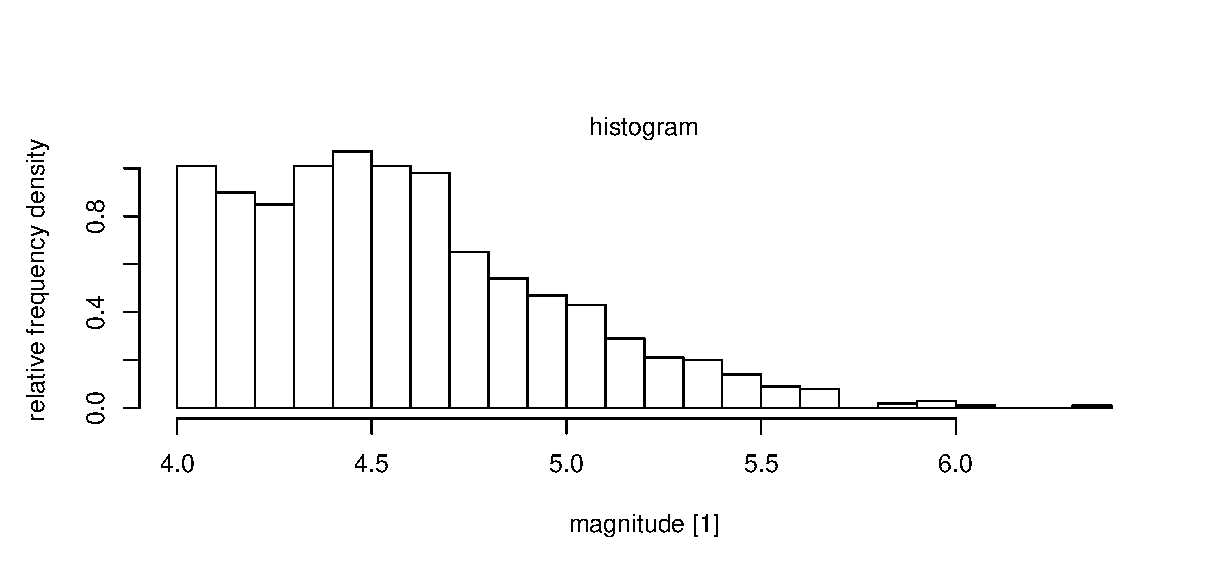
\includegraphics[scale=0.8]{histogram.eps}
\end{center}
\caption{Example of a histogram, representing the relative
frequency density for the variable ``magnitude'' in the
\R{} data set ``quakes.''
\newline
\underline{\R:} \newline
\texttt{data("quakes")} \newline
\texttt{?quakes} \newline
\texttt{hist( quakes\$mag , breaks = 20 , freq = FALSE )}}
\lb{fig:histogram}
\end{figure}
%

%
\begin{figure}[!htb]
\begin{center}
\includegraphics[scale=0.8]{barchart.eps}
\end{center}
\caption{Example of a bar chart, representing the relative
frequency distribution for the variable ``age group'' in the
\R{} data set ``esoph.'' \newline
\underline{\R:} \newline
\texttt{data("esoph")} \newline
\texttt{?esoph} \newline
\texttt{barplot( prop.table( table( esoph\$agegp ) ) )}}
\lb{fig:barchart}
\end{figure}
%

%
\begin{figure}[!htb]
\begin{flushleft}
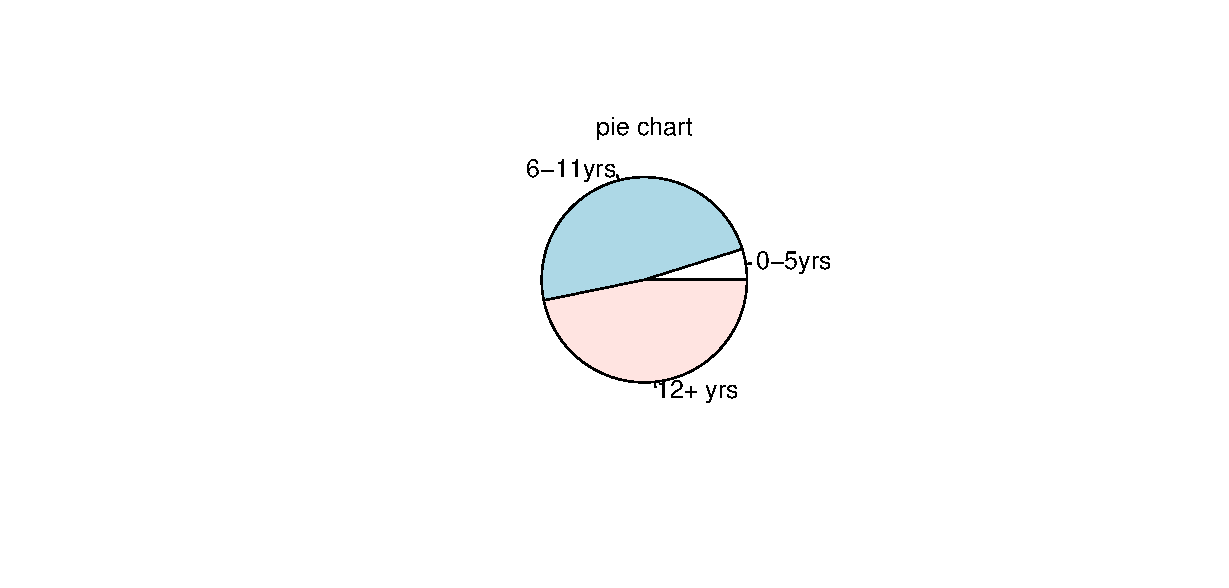
\includegraphics[scale=0.8]{piechart.eps}
\end{flushleft}
\caption{Example of a pie chart, representing the relative
frequency distribution for the variable ``education'' in the
\R{} data set ``infert.'' \newline
\underline{\R:} \newline
\texttt{data("infert")} \newline
\texttt{?infert} \newline
\texttt{pie( table( infert\$education ) )}}
\lb{fig:piechart}
\end{figure}
%

\medskip
\noindent
It is standard practice in \textbf{Statistics} to compile from the 
univariate relative frequency distribution 
$(a_{j},h_{j})_{j=1,\ldots,k}$
resp.\ $(K_{j},h_{j})_{j=1,\ldots,k}$ of data for some ordinally 
or metrically scaled one-dimensional statistical variable $X$ the 
associated empirical cumulative distribution function. Hereby it 
is necessary to distinguish the case of data for a variable with a 
discrete spectrum of values from the case of data for a variable 
with a continuous spectrum of values. We will discuss this issue 
next.

%%%%%%%%%%%%%%%%%%%%%%%%%%%%%%%%%%%%%%%%%%%%%%%%%%%%%%%%%%%%%%%%%%%
\section[Empirical cumulative distribution function (discrete
data)]{Empirical cumulative distribution function (discrete data)}
\lb{sec:empvert}
%%%%%%%%%%%%%%%%%%%%%%%%%%%%%%%%%%%%%%%%%%%%%%%%%%%%%%%%%%%%%%%%%%%
\underline{\textbf{Def.:}} Let $X$ be an ordinally or metrically
scaled one-dimensional statistical variable, the spectrum of values 
$a_{j}$ ($j=1,\ldots,k$) of which vary \textit{discretely}. Suppose 
given for $X$ a statistical sample $\boldsymbol{S_{\Omega}}$ of 
size $|\boldsymbol{S_{\Omega}}|=n$ comprising observed values 
$\{x_{i}\}_{i=1,\ldots,n}$, which we assume arranged in an 
ascending fashion according to the natural order $a_{1} < a_{2} < 
\ldots < a_{k}$. The corresponding univariate relative frequency 
distribution is $(a_{j},h_{j})_{j=1,\ldots,k}$. For all real 
numbers $x \in \mathbb{R}$, we then define by
%
\be
\lb{eq:empvert}
\fbox{$\displaystyle
F_{n}(x) :=
\begin{cases}
0 & \text{for}\ x < a_{1} \\
 & \\
{\displaystyle\sum_{i=1}^{j}h_{n}(a_{i})} & \text{for}
\ a_{j} \leq x < a_{j+1} 
\qquad (j=1,\ldots,k-1) \\
 & \\
1 & \text{for}\ x \geq a_{k}
\end{cases}
$}
\ee
%
the \textbf{empirical cumulative distribution function} for $X$.
The value of $F_{n}$ at $x \in \mathbb{R}$ represents the
cumulative relative frequencies of all $a_{j}$ which are less
or equal to $x$; cf. Fig.~\ref{fig:ecdf}. $F_{n}(x)$ has the
following properties:
%
\begin{itemize}

\item its domain is $D(F_{n})=\mathbb{R}$, and its range is 
$W(F_{n})=[0,1]$; hence, $F_{n}$ is bounded from above and from 
below,

\item it is continuous from the right and monotonously increasing,

\item it is constant on all half-open intervals $[a_{j},a_{j+1})$, 
but exhibits jump discontinuities of size $h_{n}(a_{j+1})$ at all 
$a_{j+1}$, and,

\item asymptotically, it behaves as ${\displaystyle \lim_{x\to 
-\infty}F_{n}(x)=0}$ and ${\displaystyle \lim_{x\to 
+\infty}F_{n}(x)=1}$.

\end{itemize}
%
%\textbf{"`Eichh\"ornchenmetapher"' (statistical squirrel)}: %Erstellung von $F_{n}$.

\medskip
\noindent
\underline{\R:} \texttt{ecdf(\textit{variable})},
\texttt{plot(ecdf(\textit{variable}))}

%
\begin{figure}[!htb]
\begin{flushleft}
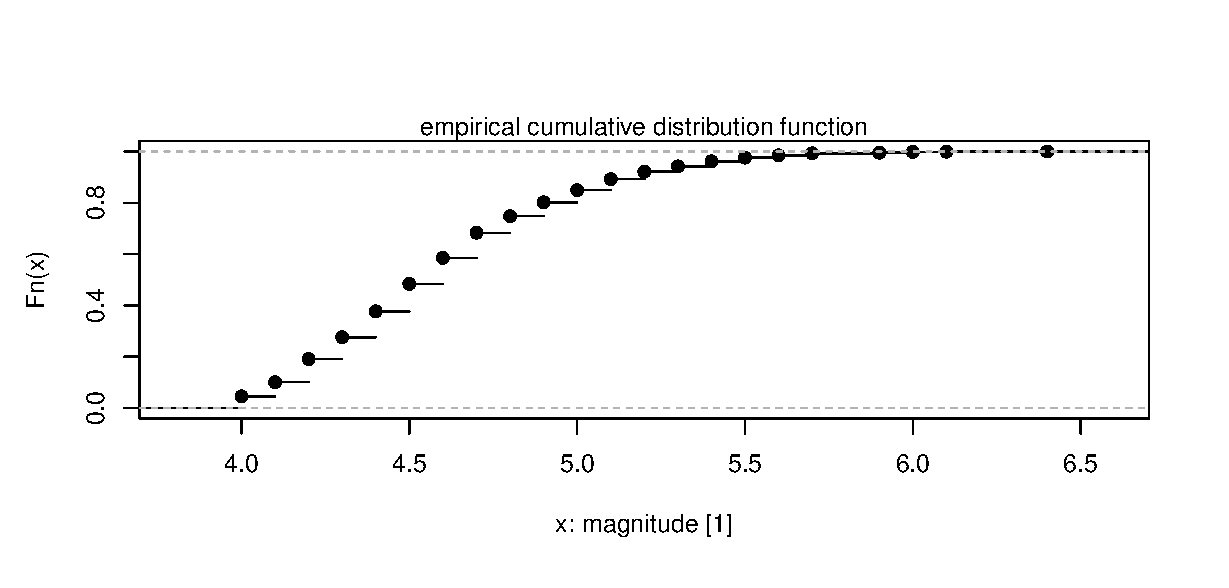
\includegraphics[scale=0.8]{empiricalcdf.eps}
\end{flushleft}
\caption{Example of an empirical cumulative distribution function,
here for the variable ``magnitude'' in the \R{} data set
``quakes.'' \newline
\underline{\R:} \newline
\texttt{data("quakes")} \newline
\texttt{?quakes} \newline
\texttt{plot( ecdf( quakes\$magnitude ) )}}
\lb{fig:ecdf}
\end{figure}
%

\medskip
\noindent
\textbf{Computational rules for} $\boldsymbol{F_{n}(x)}$

%
\begin{enumerate}
\item $h(x \leq d) = F_{n}(d)$
\item $h(x < d) = F_{n}(d) - h_{n}(d)$
\item $h(x \geq c) = 1 - F_{n}(c) + h_{n}(c)$
\item $h(x > c) =  1- F_{n}(c)$
\item $h(c \leq x \leq d) = F_{n}(d) - F_{n}(c) + h_{n}(c)$
\item $h(c < x \leq d) = F_{n}(d) - F_{n}(c)$
\item $h(c \leq x < d) = F_{n}(d) - F_{n}(c) - h_{n}(d)
+ h_{n}(c)$
\item $h(c < x < d) = F_{n}(d) - F_{n}(c) - h_{n}(d)$,
\end{enumerate}
%
wherein $c$ denotes an arbitrary \textbf{lower bound}, and $d$ 
denotes an arbitrary \textbf{upper bound}, on the argument $x$ of 
$F_{n}(x)$.

%%%%%%%%%%%%%%%%%%%%%%%%%%%%%%%%%%%%%%%%%%%%%%%%%%%%%%%%%%%%%%%%%%%
\section[Empirical cumulative distribution function (continuous
data)]{Empirical cumulative distribution function (continuous
data)}
\lb{empvertklass}
%%%%%%%%%%%%%%%%%%%%%%%%%%%%%%%%%%%%%%%%%%%%%%%%%%%%%%%%%%%%%%%%%%%
\underline{\textbf{Def.:}} Let $X$ be a metrically scaled
one-dimensional statistical variable, the spectrum of values of 
which vary \textit{continuously}, and let observed values 
$\{x_{i}\}_{i=1,\ldots,n}$ for $X$ from a statistical sample 
$\boldsymbol{S_{\Omega}}$ of size $|\boldsymbol{S_{\Omega}}|=n$ be 
binned into a finite set of $k$ (with $k \approx \sqrt{n}$) 
ascendingly ordered exclusive \textbf{class intervals} (or bins) 
$K_{j}$ ($j=1,\ldots,k$), of width $b_{j}$, and with lower 
boundary~$u_{j}$ and upper boundary~$o_{j}$. The univariate 
distribution of relative frequencies of the class intervals be 
$(K_{j},h_{j})_{j=1,\ldots,k}$. Then, for all real numbers $x \in 
\mathbb{R}$,
%
\be
\lb{klempvert}
\fbox{$\displaystyle
\tilde{F}_{n}(x) :=
\begin{cases}
0 & \text{for}\ x< u_{1} \\
 & \\
{\displaystyle \sum_{i=1}^{j-1}h_{i}
+ \frac{h_{j}}{b_{j}}(x-u_{j})}
& \text{for}\ x \in K_{j} \\
 & \\
1 & \text{for}\ x > o_{k}
\end{cases}
$}
\ee
%
defines the \textbf{empirical cumulative distribution function}
for $X$. $\tilde{F}_{n}(x)$ has the following properties:
%
\begin{itemize}

\item its domain is $D(\tilde{F}_{n})=\mathbb{R}$, and its
range is $W(\tilde{F}_{n})=[0,1]$; hence, $\tilde{F}_{n}$ is 
bounded from above and from below,

\item it is continuous and monotonously increasing, and,

\item asymptotically, it behaves as ${\displaystyle\lim_{x\to 
-\infty}\tilde{F}_{n}(x)=0}$ and ${\displaystyle\lim_{x\to 
+\infty}\tilde{F}_{n}(x)=1}$.
\end{itemize}
%

\medskip
\noindent
\underline{\R:} \texttt{ecdf(\textit{variable})},
\texttt{plot(ecdf(\textit{variable}))}

\medskip
\noindent
\textbf{Computational rules for} $\boldsymbol{\tilde{F}_{n}(x)}$
%
\begin{enumerate}

\item $h(x<d)=h(x\leq d) = \tilde{F}_{n}(d)$

\item $h(x>c)=h(x\geq c) = 1-\tilde{F}_{n}(c)$

\item $h(c<x<d) = h(c\leq x<d) = h(c<x\leq d)
= h(c\leq x\leq d) = \tilde{F}_{n}(d)-\tilde{F}_{n}(c)$,
\end{enumerate}
%
wherein $c$ denotes an arbitrary \textbf{lower bound}, and $d$ 
denotes an arbitrary \textbf{upper bound}, on the argument $x$ of
$\tilde{F}_{n}(x)$.

\vspace{5mm}
\noindent
Our next steps comprise the introduction of a set of 
scale-level-dependent standard \textbf{descriptive measures} which 
characterise specific properties of univariate and bivariate 
relative frequency distributions of statistical variables $X$ 
resp.\ $(X,Y)$.

%%%%%%%%%%%%%%%%%%%%%%%%%%%%%%%%%%%%%%%%%%%%%%%%%%%%%%%%%%%%%%%%%%%
%%%%%%%%%%%%%%%%%%%%%%%%%%%%%%%%%%%%%%%%%%%%%%%%%%%%%%%%%%%%%%%%%%%
